\documentclass{standalone}
\usepackage{tikz}
\usetikzlibrary{patterns, positioning}


\begin{document}
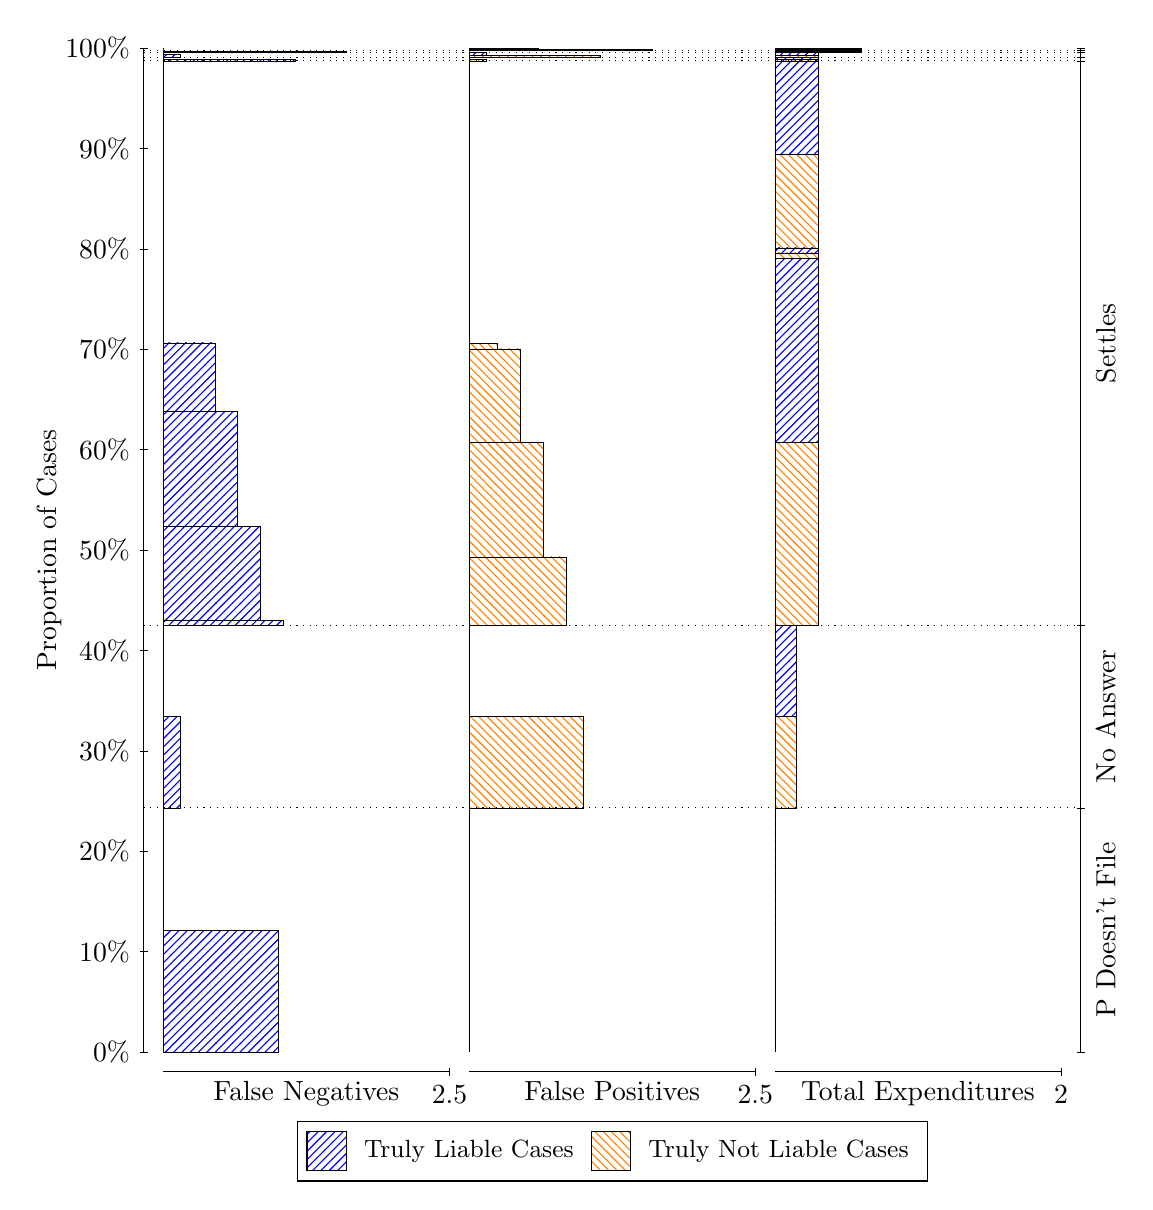
\begin{tikzpicture}
\draw[black, very thin] (1.5,1.75) -- (1.5,14.5);
\node[rotate=90, text=black, anchor=center] at (0.3, 8.125) {Proportion of Cases};
\draw[black, very thin] (1.45,1.75) -- (1.55,1.75);
\node[text=black, anchor=east] at (1.45, 1.75) {0\%};
\draw[black, very thin] (1.45,3.025) -- (1.55,3.025);
\node[text=black, anchor=east] at (1.45, 3.025) {10\%};
\draw[black, very thin] (1.45,4.3) -- (1.55,4.3);
\node[text=black, anchor=east] at (1.45, 4.3) {20\%};
\draw[black, very thin] (1.45,5.575) -- (1.55,5.575);
\node[text=black, anchor=east] at (1.45, 5.575) {30\%};
\draw[black, very thin] (1.45,6.85) -- (1.55,6.85);
\node[text=black, anchor=east] at (1.45, 6.85) {40\%};
\draw[black, very thin] (1.45,8.125) -- (1.55,8.125);
\node[text=black, anchor=east] at (1.45, 8.125) {50\%};
\draw[black, very thin] (1.45,9.4) -- (1.55,9.4);
\node[text=black, anchor=east] at (1.45, 9.4) {60\%};
\draw[black, very thin] (1.45,10.675) -- (1.55,10.675);
\node[text=black, anchor=east] at (1.45, 10.675) {70\%};
\draw[black, very thin] (1.45,11.95) -- (1.55,11.95);
\node[text=black, anchor=east] at (1.45, 11.95) {80\%};
\draw[black, very thin] (1.45,13.225) -- (1.55,13.225);
\node[text=black, anchor=east] at (1.45, 13.225) {90\%};
\draw[black, very thin] (1.45,14.5) -- (1.55,14.5);
\node[text=black, anchor=east] at (1.45, 14.5) {100\%};

\draw[black, very thin] (13.4,1.75) -- (13.4,14.5);
\draw[black, very thin] (13.35,1.75) -- (13.45,1.75);
\node[anchor=west] at (13.35, 1.75) {};
\draw[black, very thin] (13.35,4.8497) -- (13.45,4.8497);
\node[anchor=west] at (13.35, 4.8497) {};
\draw[black, very thin] (13.35,7.1679) -- (13.45,7.1679);
\node[anchor=west] at (13.35, 7.1679) {};
\draw[black, very thin] (13.35,14.336) -- (13.45,14.336);
\node[anchor=west] at (13.35, 14.336) {};
\draw[black, very thin] (13.35,14.384) -- (13.45,14.384);
\node[anchor=west] at (13.35, 14.384) {};
\draw[black, very thin] (13.35,14.442) -- (13.45,14.442);
\node[anchor=west] at (13.35, 14.442) {};
\draw[black, very thin] (13.35,14.471) -- (13.45,14.471);
\node[anchor=west] at (13.35, 14.471) {};
\draw[black, very thin] (13.35,14.5) -- (13.45,14.5);
\node[anchor=west] at (13.35, 14.5) {};

\draw[black, very thin, pattern color=blue, pattern=north east lines] (1.75,1.75) rectangle (3.2033,3.2894);
\draw[black, very thin, pattern color=orange, pattern=north west lines] (1.75,3.2894) rectangle (1.75,4.8497);
\draw[black, very thin, pattern color=blue, pattern=north east lines] (1.75,4.8497) rectangle (1.968,6.0088);
\draw[black, very thin, pattern color=orange, pattern=north west lines] (1.75,6.0088) rectangle (1.75,7.1679);
\draw[black, very thin, pattern color=blue, pattern=north east lines] (1.75,7.1679) rectangle (3.276,7.2326);
\draw[black, very thin, pattern color=blue, pattern=north east lines] (1.75,7.2326) rectangle (2.9853,8.4229);
\draw[black, very thin, pattern color=blue, pattern=north east lines] (1.75,8.4229) rectangle (2.6947,9.8851);
\draw[black, very thin, pattern color=blue, pattern=north east lines] (1.75,9.8851) rectangle (2.404,10.754);
\draw[black, very thin, pattern color=orange, pattern=north west lines] (1.75,10.754) rectangle (1.75,14.336);
\draw[black, very thin, pattern color=blue, pattern=north east lines] (1.75,14.336) rectangle (3.4213,14.36);
\draw[black, very thin, pattern color=orange, pattern=north west lines] (1.75,14.36) rectangle (1.75,14.384);
\draw[black, very thin, pattern color=blue, pattern=north east lines] (1.75,14.384) rectangle (1.968,14.419);
\draw[black, very thin, pattern color=orange, pattern=north west lines] (1.75,14.419) rectangle (1.75,14.442);
\draw[black, very thin, pattern color=blue, pattern=north east lines] (1.75,14.442) rectangle (4.0753,14.456);
\draw[black, very thin, pattern color=orange, pattern=north west lines] (1.75,14.456) rectangle (1.75,14.471);
\draw[black, very thin, pattern color=orange, pattern=north west lines] (1.75,14.471) rectangle (1.75,14.483);
\draw[black, very thin, pattern color=blue, pattern=north east lines] (1.75,14.483) rectangle (1.75,14.5);
\draw[black, very thin, pattern color=orange, pattern=north west lines] (5.6333,1.75) rectangle (5.6333,3.3102);
\draw[black, very thin, pattern color=blue, pattern=north east lines] (5.6333,3.3102) rectangle (5.6333,4.8497);
\draw[black, very thin, pattern color=orange, pattern=north west lines] (5.6333,4.8497) rectangle (7.0867,6.0088);
\draw[black, very thin, pattern color=blue, pattern=north east lines] (5.6333,6.0088) rectangle (5.6333,7.1679);
\draw[black, very thin, pattern color=orange, pattern=north west lines] (5.6333,7.1679) rectangle (6.8687,8.0372);
\draw[black, very thin, pattern color=orange, pattern=north west lines] (5.6333,8.0372) rectangle (6.578,9.4955);
\draw[black, very thin, pattern color=orange, pattern=north west lines] (5.6333,9.4955) rectangle (6.2873,10.679);
\draw[black, very thin, pattern color=orange, pattern=north west lines] (5.6333,10.679) rectangle (5.9967,10.749);
\draw[black, very thin, pattern color=blue, pattern=north east lines] (5.6333,10.749) rectangle (5.6333,14.336);
\draw[black, very thin, pattern color=orange, pattern=north west lines] (5.6333,14.336) rectangle (5.8513,14.36);
\draw[black, very thin, pattern color=blue, pattern=north east lines] (5.6333,14.36) rectangle (5.6333,14.384);
\draw[black, very thin, pattern color=orange, pattern=north west lines] (5.6333,14.384) rectangle (7.3047,14.407);
\draw[black, very thin, pattern color=blue, pattern=north east lines] (5.6333,14.407) rectangle (5.8513,14.442);
\draw[black, very thin, pattern color=orange, pattern=north west lines] (5.6333,14.442) rectangle (5.6333,14.457);
\draw[black, very thin, pattern color=blue, pattern=north east lines] (5.6333,14.457) rectangle (5.6333,14.471);
\draw[black, very thin, pattern color=orange, pattern=north west lines] (5.6333,14.471) rectangle (7.9587,14.483);
\draw[black, very thin, pattern color=blue, pattern=north east lines] (5.6333,14.483) rectangle (6.5053,14.5);
\draw[black, very thin, pattern color=orange, pattern=north west lines] (9.5167,1.75) rectangle (9.5167,3.3102);
\draw[black, very thin, pattern color=blue, pattern=north east lines] (9.5167,3.3102) rectangle (9.5167,4.8497);
\draw[black, very thin, pattern color=orange, pattern=north west lines] (9.5167,4.8497) rectangle (9.7892,6.0088);
\draw[black, very thin, pattern color=blue, pattern=north east lines] (9.5167,6.0088) rectangle (9.7892,7.1679);
\draw[black, very thin, pattern color=orange, pattern=north west lines] (9.5167,7.1679) rectangle (10.062,9.4955);
\draw[black, very thin, pattern color=blue, pattern=north east lines] (9.5167,9.4955) rectangle (10.062,11.827);
\draw[black, very thin, pattern color=orange, pattern=north west lines] (9.5167,11.827) rectangle (10.062,11.897);
\draw[black, very thin, pattern color=blue, pattern=north east lines] (9.5167,11.897) rectangle (10.062,11.962);
\draw[black, very thin, pattern color=orange, pattern=north west lines] (9.5167,11.962) rectangle (10.062,13.146);
\draw[black, very thin, pattern color=blue, pattern=north east lines] (9.5167,13.146) rectangle (10.062,14.336);
\draw[black, very thin, pattern color=orange, pattern=north west lines] (9.5167,14.336) rectangle (10.062,14.36);
\draw[black, very thin, pattern color=blue, pattern=north east lines] (9.5167,14.36) rectangle (10.062,14.384);
\draw[black, very thin, pattern color=orange, pattern=north west lines] (9.5167,14.384) rectangle (10.062,14.407);
\draw[black, very thin, pattern color=blue, pattern=north east lines] (9.5167,14.407) rectangle (10.062,14.442);
\draw[black, very thin, pattern color=orange, pattern=north west lines] (9.5167,14.442) rectangle (10.607,14.457);
\draw[black, very thin, pattern color=blue, pattern=north east lines] (9.5167,14.457) rectangle (10.607,14.471);
\draw[black, very thin, pattern color=orange, pattern=north west lines] (9.5167,14.471) rectangle (10.607,14.483);
\draw[black, very thin, pattern color=blue, pattern=north east lines] (9.5167,14.483) rectangle (10.607,14.5);
\draw[black, dotted] (1.5,4.8497) -- (13.4,4.8497);
\draw[black, dotted] (1.5,7.1679) -- (13.4,7.1679);
\draw[black, dotted] (1.5,14.336) -- (13.4,14.336);
\draw[black, dotted] (1.5,14.384) -- (13.4,14.384);
\draw[black, dotted] (1.5,14.442) -- (13.4,14.442);
\draw[black, dotted] (1.5,14.471) -- (13.4,14.471);
\draw[black, very thin] (1.75,1.5) -- (5.3833,1.5);
\node[text=black, anchor=north] at (3.5667, 1.5) {False Negatives};
\draw[black, very thin] (5.3833,1.45) -- (5.3833,1.55);
\node[text=black, anchor=north] at (5.3833, 1.45) {2.5};

\draw[black, very thin] (5.6333,1.5) -- (9.2667,1.5);
\node[text=black, anchor=north] at (7.45, 1.5) {False Positives};
\draw[black, very thin] (9.2667,1.45) -- (9.2667,1.55);
\node[text=black, anchor=north] at (9.2667, 1.45) {2.5};

\draw[black, very thin] (9.5167,1.5) -- (13.15,1.5);
\node[text=black, anchor=north] at (11.333, 1.5) {Total Expenditures};
\draw[black, very thin] (13.15,1.45) -- (13.15,1.55);
\node[text=black, anchor=north] at (13.15, 1.45) {2};

\node[text=black, centered, rotate=90] at (13.72, 3.2998) {P Doesn't File};
\node[text=black, centered, rotate=90] at (13.72, 6.0088) {No Answer};
\node[text=black, centered, rotate=90] at (13.72, 10.752) {Settles};





\draw (7.449999999999999,1.5) node[draw=none] (baseCoordinate) {};
\begin{scope}[align=center]
        \matrix[scale=0.5, draw=black, below=0.5cm of baseCoordinate, nodes={draw}, column sep=0.1cm]{
            \node[rectangle, draw, minimum width=0.5cm, minimum height=0.5cm, pattern color=blue, pattern=north east lines] {}; &
            \node[draw=none, font=\small, text=black] (B) {Truly Liable Cases}; &
            \node[rectangle, draw, minimum width=0.5cm, minimum height=0.5cm, pattern color=orange, pattern=north west lines] {}; &
            \node[draw=none, font=\small, text=black] (B) {Truly Not Liable Cases}; \\
            };
\end{scope}

\end{tikzpicture}
\end{document}